\chapter{Critical Evaluation}
\label{chap:evaluation}

\section{Analysis of Word Lists}
\begin{figure}[ht]
\begin{subfigure}[b]{\textwidth}
\centering
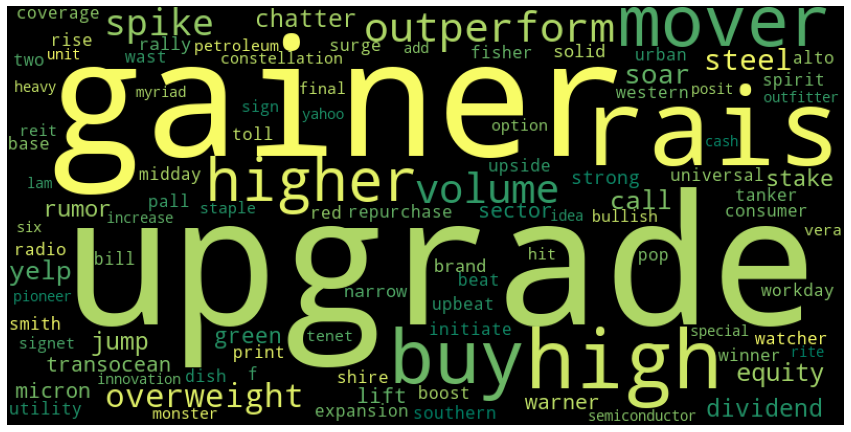
\includegraphics[scale=0.4]{pics/positive.png}
\caption{Positive words}
\end{subfigure}

\begin{subfigure}[b]{\textwidth}
\centering
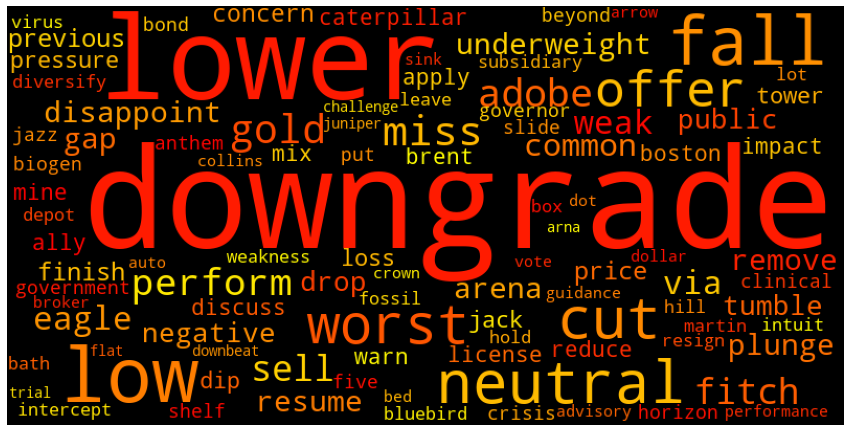
\includegraphics[scale=0.4]{pics/negative.png}
\caption{Negative words}
\end{subfigure}
\caption[Word clouds]{Word clouds demonstrating sentiment charged words. Font size corresponds to average tone across all training samples}
\label{wordclouds}
\end{figure}

Following the construction of matrix $O$, figure \ref{wordclouds} demonstrates the list of sentiment charged words on average over all training 19 windows. At each training and validation window, the sentiment lists are generated completely from scratch, and while there is some overlap, each list can vary significantly. The font size corresponds to the average tone (calculated by $\frac{1}{2}(O_+ - O_-)$) of the words across all windows. Of the top 50 positive sentiment words, the following appeared in at least 15 of the 19 windows, with words highlighted in \textbf{bold} appearing in all windows:
\begin{center}
      \textit{author, rumor, volume, repurchase, rais(e),} \textbf{gainer, mover, high, upgrade}
\end{center}

\noindent
The following words appear in at least 15 of the 19 windows with respect to top 50 negative sentiment words with those highlighted in \textbf{bold} appearing in all windows:
\begin{center}
      \textit{offer, negative, neutral, public, low,} \textbf{miss, lower, loser, cut, fall, weak downgrade, underweight}
\end{center}

Simply by inspection, each group appears reasonable, in the sense that many of the words with high values in either sentiment could be assumed. However, some words are somewhat surprising and this may offer an insight into subconscious bias that exists in writing headlines as opposed to article bodies. For example, the word \textit{volume} is, under normal circumstances, a sentiment neutral word, but according to the model generated by SESTM, is a highly positive word. Examples of headlines including this word include:
\begin{itemize}
      \item \textit{Agilent spikes to high of \$60.40 on Volume}
      \item \textit{Markets gather some momentum as volume remains light, geopolitical tension improving}
      \item \textit{Tuesday's Mid-day options for volume leaders}
\end{itemize}

Observing these headlines, it is clear that the words are being used in a positive context, and this could be due to subconscious usage of the word when constructing such headlines. However, another explanation could be overfitting. Included in the sample are headlines from `Benzinga', which is a company that offers realtime news articles, and has a significant quantity of headlines of the form \textit{Benzinga's top upgrades} (around 16,000 headlines from the entire dataset) and \textit{Benzinga's volume} (with around 2,000). This could be seen as an issue of overfitting and may skew these words' sentiment value meaning that it is not reflective of the true sentiment of the word when not used in the context of Benzinga. However, both `upgrade' and `volume' appear multiple times in the word lists for bigrams with different combinations of words, meaning that there is positive sentiment attached to these words without the context of Benzinga.

Some words, such as `rais' are cut off to their stem by the stemming and lemmatisation step (i.e. `rais' from `raise'), as the stem is also an English word. However, such words are likely to be very infrequently used words themselves, and are very unlikely to be used in a headline. These edge cases do not affect the overall predictive quality of the model, as evidenced by the words shown in figure \ref{wordclouds}. The sentiment for each word is still captured in the stem, and each article is processed in the same way, thus there is no sentiment or predictive power lost in this way. There is a slight complication when it comes to comparing the words included in the model to those in the H4 and LM lexicons, as these lexicons do not contain the stemmed words. For this reason, when checking if a word in the trained model exists in either dictionary, each word in either dictionary is preprocessed in the same way discussed in section \ref{sec:pre-processing}

When compared to the Harvard IV and Loughran McDonald dictionaries, we find that the majority of words labelled with sentiment according to our model are not in either dictionary. The negative sentiment words have much higher overlap, with 13 of the top 50 words appearing in the LM dictionary, while only 3 appear in the H4. Conversely, only 6 words overlap LM in the positive tone, while 5 words overlap the H4 dictionary. Furthermore, many words that are included in either dictionary are determined to be sentiment neutral by the model. This is because the model is trained on a sample of headlines and the vocabulary used in headlines is vastly different to that in everyday use or 10-k filings in the case of LM. Headline vocabulary often contains much more impactful words, as it is intended to be a punchy, attention grabbing piece of text. Often, words that are typically used in headlines are rarely found outside of the context of headlines \parencite{language-newspapers}. For this reason, the lexicons of the model, and that of H4 and LM differ significantly.

\subsection{Bigrams}
The order in which words appear in can have a profound effect on the sentiment of a word. This order sentiment can be captured by exploring the dictionary when constructed from \textit{bigrams} as opposed to unigrams alone. By combining both of these dictionaries, it is possible to gain a clearer understanding of the true sentiment of a headline. Many of the frequently  words unigrams also appear in the bigram. This is partly due to the mutual information restriction on the bigrams consiered by the model, but also because still carry sentiment in combination with other words. Furthermore, somewhat surprisingly there are bigrams that appear in every training window. The headlines in this dataset have an average wordcount of 6.11 (excluding stopwords and non-English words), and therefore one may expect that there would be very few repeating bigrams, which is not the case. This signifies that headline writers may subconsciously use certain combinations of words to convey either positive or negative sentiment

The following bigrams appear positively in at least 13 of the 19 training windows, with those highlighted in \textbf{bold} appearing in all headlines:
\begin{center}
\textit{micron technology, repurchase program, spike higher,} \textbf{volume mover}, \textbf{week high}
\end{center}

The following bigrams appear negatively in at least 14 of the 19 training windows, with those highlighted in \textbf{bold} appearing in all headlines:
\begin{center}
      \textit{general dynamic, bath beyond, bed bath, sector perform, secondary offer, week low, resume trade, offer common,} \textbf{public offer}
\end{center}



\section{Daily returns}


\begin{table}[!ht]
\begin{center}
\begin{tabular}{lccccccc}
      \toprule
      & Sharpe &  Average & Daily & \multicolumn{2}{c}{FF3} & \multicolumn{2}{c}{FF5} \\
      \cmidrule(lr){5-6}
      \cmidrule(lr){7-8}
      % \cmidrule(lr){9-10}
      Formation & Ratio & Return & Turnover & $\alpha$ & $R^2$ & $\alpha$ & $R^2$ \\
      \midrule
      EW LS & 0.84 & 9.23 & & 5.59 & 4.11\% & 5.57 & 4.16\% \\
      EW L & 0.69 & 9.75 & & 6.56 & 21.62\% & 5.86 & 23.0\% \\
      EW S & -0.09 & -0.53 & & -1.66 & 25.71\% & -0.98 & 26.68\% \\
      VW LS & 0.98 & 8.37 & & 6.63 & 5.74\% & 7.04 & 7.12\% \\
      VW L & 0.33 & 3.95 & & 1.38 & 27.93\% & 1.17 & 28.64\% \\
      VW S & 0.31 & 4.41 & & 4.55 & 31.78\% & 5.18 & 33.82\% \\
      \bottomrule
\end{tabular}
\caption{Performance of Daily News Sentiment Portfolios one day ahead}
\label{portfolio-performance}
\end{center}
\end{table}

Using the headlines that were saved for out of sample testing, a portfolio is constructed for each day. On average, 358 firms have articles linked to them on a given day, and of these, almost three quarters of these firms have headlines containing one or more sentiment words (are not marked neutral by the model). According to the constraints ($\widehat p_i < 0.5$ for a stock to be bought, and vice versa for a stock to be sold), there are some days where less than 100 stocks form the portfolio, in which case we trade with the largest value possible. On average, the long side of the portfolio has 40 stocks, while the short side has 48, therefore the average number of stocks in the portfolio is 88.

Table \ref{portfolio-performance} describes the performance of the constructed portfolios. The long-short portfolio is a zero-net-investment portfolio, which is a theoretical portfolio that requires zero investment, as it buys the same value of stocks as it sells \parencite{zero-net}. The portfolio is theoretical as a true zero-cost investment is impossible in practice for a number of reasons, one of which being that to sell a stock and profit from the decline, there is collateral from the loan from the broker. However, for the purposes of the following experiments, it is sufficient. The two investment methods (equal and value weighted) are split up into the long-short combined portfolio (L-S), and the long (L) and short (S) legs are also displayed separately for comparison purposes. The daily turnover section displays the average turnover each day, which would be 100\% as the profit is liquidated at the end of each day, but some stocks are retained the following day. A turnover of 90\% (as in VW L) implies that on average 1 in 10 stocks are retained the following day. This could be due to headlines or news articles that are concerning the same events (stale news), or repeat sentiment headlines as a story unfolds over a number of days.

The sharpe ratio refers to the calculated annualised sharpe ratio and this reflects the ratio of profit versus risk. This is then annualised by multiplying the daily sharpe ratio (shown in \ref{ssub:sharpe-ratio}) by $\sqrt{252}$ as this is the number of trading days in a year, and will give a clearer image of the risk involved in the potential profit.

The FF3 and FF5 sections refer to Fama French 3 and 5 factor regression respectively, while the $\alpha$ concerns the intercept. This reflects how much the output outperformed the expected value calculated by the factors in the model. This alpha is generated by privately created information, or information that is not available in the market. In other words, if the $\alpha$ is a very small percentage of the generated returns, then the returns that an investment has generated can be explained by regular movement in the markets, and there is no private information that is being used to generate profit. The $R^2$ value is the measure of the proportion of variance that is for the dependent variable (in this case, daily returns for the portfolio) is explained by the independent variables (in this case, the Fama French factors discussed in \ref{ssub:fama-french}). Therefore, if $R^2 = 25\%$, then around a quarter of the observed variation can be explained by the inputs. In terms of an investment, this corresponds to the percentage of movement that can be explained by movements in the independent variables.

This figure clarifies identifies three key facts: firstly, most of the formations generate a slight profit with a fair amount of risk, reflected in the Sharpe ratios. None of the formations have a Sharpe ratio of $>1$, meaning each of the portfolios carry significant risk. The second fact that the equal weighted formation outperforms the value weighted formation slightly overall, with slightly higher risk, while the value weighted section carries the least risk relative to profit. The equal weighted portfolio outperforms value weighted slightly in the long leg, while the short leg favours the value weighted formation significantly. Fundamentally, this means that the trained model is better at detecting positive sentiment about smaller stocks than that of larger stocks, while also being better at detecting negative sentiment in larger stocks than smaller stocks. This is likely due to the nature of headlines as, while they are intended to summarise the contents of a news article, the language used favours information that is likely to generate clicks and views. Small stocks performing well and large, supposedly stable stocks performing poorly are more likely to incentivise a user to click on the full article than their respective counterparts, meaning these are more likely to be included in the headline itself. Additionally,  Furthermore, the risk of the market lies with the party who shorts a stoc %todo: continue this explanation

\begin{figure}[!t]
      \centering
\begin{tikzpicture}
\begin{axis}[scale only axis, height=8cm, width=\textwidth*.9, grid=both,
      legend pos=north west,
      date coordinates in=x, date ZERO=2019-01-01, xticklabel=\month-\year,ymin=-50,ymax=75,
      xtick={2019-01-01,2019-02-01,2019-03-01,2019-04-01,2019-05-01,2019-06-01,2019-07-01,2019-08-01,2019-09-01,2019-10-01,2019-11-01,2019-12-01,2020-01-01,2020-02-01,2020-03-01,2020-04-01,2020-05-01,2020-06-01},
      xticklabel style={
            rotate=60,
      },
       xmin=2019-01-01,
       xmax=2020-06-08]
\addplot [red, very thick, mark=none] table [header=true,x=date,y=EW-L, col sep=comma]{data/one-day-ahead.csv};
\addplot [blue, very thick, mark=none] table [header=true,x=date,y=EW-S, col sep=comma]{data/one-day-ahead.csv};
\addplot [black, very thick, mark=none] table [header=true,x=date,y=EW-LS, col sep=comma]{data/one-day-ahead.csv};
\addplot [red, very thick, dotted, mark=none] table [header=true,x=date,y=VW-L, col sep=comma]{data/one-day-ahead.csv};
\addplot [blue, very thick, dotted, mark=none] table [header=true,x=date,y=VW-S, col sep=comma]{data/one-day-ahead.csv};
\addplot [black, very thick, dotted, mark=none] table [header=true,x=date,y=VW-LS, col sep=comma]{data/one-day-ahead.csv};
% \draw ({axis cs:2020-03-11,0}|-{rel axis cs:0,0}) -- ({axis cs:2020-03-11,0}|-{rel axis cs:0,1})
 \draw[green, very thick] (axis cs: 2020-03-11,\pgfkeysvalueof{/pgfplots/ymin}) -- 
                      (axis cs: 2020-03-11,\pgfkeysvalueof{/pgfplots/ymax})node[anchor=west,rotate=90]{Coronavirus declard pandemic};
                
\legend{L EW, S EW, LS EW, L VW, S VW, LS VW}

\end{axis}
\end{tikzpicture}
\caption[Daily cumulative log returns]{Cumulative log returns for each formation over the out of sample headlines}
\label{graph-returns}
\end{figure}


Figure \ref{graph-returns} details the cumulative log returns over the entire out of sample dataset. Here, The performance of each of the legs are relatively steady in their respective directions until March 2020. At this point, the profits of the short legs skyrocket, while that of the long section plummet --- especially for the value weighted portfolios. This is due to the Coronavirus outbreak, as it was officially declared a pandemic on March 11 2020, indicted by the vertical green line on the graph. Due to lockdown restrictions imposed wordwode, the stock market experienced one of the worst crashes, and was felt particularly by large stocks, before recovering a short while later. The markets began feeling the effect of the lockdown in February 2020, and the crash peaked in March 2020, before beginning to recover in late April \parencite{covid-impact}. This crash can be clearly seen in the affected profits, as the long side suffers significantly, while the short side succeeds greatly. This is simply due to the vasy majority of stocks falling in value, therefore shorting almost any stocks during this time would result in a profit. The extreme disparity in profit for the long side also clearly highlights a limitation with all lexicon based sentiment analysis methods, whether they use supervised learning signals, or use a manually labelled dictionary: they are unable to adapt to rapid changes. Since the COVID-19 virus did not exist during the training and validation samples, the model has no information on the sentiment of headlines that would discuss this, and would ignore it. Naturally, if the model was retrained using data from this time period, it would be able to detect such headlines in the future, but the crux of the issue is that it is impossible to obtain enough information to allow the model to react to such drastic changes in the market.

\begin{table}[!ht]
\begin{center}
\begin{tabular}{lccccccc}
      \toprule
      & Sharpe &  Average & Daily & \multicolumn{2}{c}{FF3} & \multicolumn{2}{c}{FF5} \\
      \cmidrule(lr){5-6}
      \cmidrule(lr){7-8}
      Formation & Ratio & Return & Turnover & $\alpha$ & $R^2$ & $\alpha$ & $R^2$ \\
      \midrule
EW LS & 0.66 & 6.51 & & 5.52 & 2.24\% & 4.16 & 4.51\% \\
EW L & 0.64 & 5.46 & & 1.95 & 9.67\% & 0.58 & 12.97\% \\
EW S & 0.03 & 1.05 & & 2.76 & 16.16\% & 2.77 & 16.96\% \\
VW LS & 0.03 & 0.98 & & 0.93 & 2.56\% & 0.75 & 2.66\% \\
VW L & -0.37 & -1.58 & & -4.67 & 14.12\% & -5.13 & 14.62\% \\
VW S & 0.25 & 2.56 & & 4.79 & 21.41\% & 5.07 & 21.56\% \\
      \bottomrule
\end{tabular}
\caption{Performance of Daily News Sentiment Portfolios one day ahead, ignoring headlines dated after January 2020}
\label{tab:portfolio-performance-no-covid}
\end{center}
\end{table}

For better analysis of the model's predictive ability, table \ref{tab:portfolio-performance-no-covid} shows the same metrics as table \ref{portfolio-performance}, only without any of the out of sample articles dated after January 2020 to observe the impact without the greatly added noise of a stock market crash. Here, the trend of the data is very similar, with the equal weighted long formation still outperforming its value weighting counterpart, and vice versa with the short side, meaning that it remains steadfast that headlines indicating negative sentiment about larger stocks contain more reliable information than that with positive stocks. All formations perform slightly worse, with the short side of the value weighted being the only formation that retains the majority of its profit and risk. All Sharpe ratios are also lower, indicating higher risk. The changes here are due to the extreme values on either side of the market crash skewing the averages, and once this is removed, a clearer image of how the model would perform under normal circumstances. As such, it is clear that the model struggles somewhat to see any profit devoid of any serious risk. Using headlines as a method from which to extract data is significantly harder than that of longer texts, since the frequency of sentiment words is very low. There are only likely to be one or two sentiment words in any given headline due to the naturally low word count, and as such the conclusions drawn from this data contains large room for error, which explains the lack of profit. There is still some information to be gained, but this signal is not as clear as other text forms.


\begin{table}[!ht]
\begin{center}
\begin{tabular}{lccccccc}
      \toprule
      & Sharpe &  Average & Daily & \multicolumn{2}{c}{FF3} & \multicolumn{2}{c}{FF5} \\
      \cmidrule(lr){5-6}
      \cmidrule(lr){7-8}
      % \cmidrule(lr){9-10}
      Formation & Ratio & Return & Turnover & $\alpha$ & $R^2$ & $\alpha$ & $R^2$ \\
      \midrule
      EW LS & 1.75 & 20.69 & & 18.19 & 8.87\% & 17.71 & 8.98\% \\
      EW L & 1.29 & 17.84 & & 14.55 & 18.81\% & 14.02 & 19.93\% \\
      EW S & 0.15 & 2.85 & & 2.95 & 34.48\% & 3.0 & 35.2\% \\
      VW LS & 0.9 & 8.09 & & 6.85 & 5.71\% & 7.29 & 6.31\% \\
      VW L & 0.68 & 7.43 & & 4.95 & 29.62\% & 4.97 & 30.64\% \\
      VW S & -0.0 & 0.66 & & 1.21 & 35.07\% & 1.63 & 36.71\% \\
      \bottomrule
\end{tabular}
\caption[Day ahead performance different configurations]{Performance of daily news sentiment portfolios using different configurations}
\label{tab:other-configs-day-ahead}
\end{center}
\end{table}

Table \ref{tab:other-configs-day-ahead} shows the performance of the portfolios under differing conditions. Most notable in this table is the vast improvement in performance that augmenting the sentiment word list with bigrams has on both the sharpe ratios and the average daily returns, particularly in both long legs of the portfolios. The only formation that suffers from this modification is the short side of the value weighted portfolio. The sharpe ratio of 1.75 produced by the equal weighted portfolio shows that the profit generated has a very favourable risk to profit ratio. This shift in performance indicates that positive sentiment in headlines is often conveyed over multiple words, rather than single words. The inverse is true for negative sentiment, as the equal short leg slightly benefits from the introduction of bigrams, and the value weighted short leg is harmed by this introduction. This data does contradict the idea that negative news about larger stocks is more reliable than that of smaller stocks, due to the outperformance of the equal weighted short leg to the value weighted.


%note!: alpha for 

%todo: do portfolios trading 200 stocks also to show robustness
\section{Speed of information Assimilation}

In the previous sections, we explore the relationship between the sentiment score of a headline calculated by the model and the changes in price the following day. Here, we explore the relationship between the changes in price after differing delays to investigate timing responses.

\begin{table}[!t]
\begin{center}
\begin{tabular}{lccccccc}
      \toprule
      & Sharpe &  Average & Daily & \multicolumn{2}{c}{FF3} & \multicolumn{2}{c}{FF5} \\
      \cmidrule(lr){5-6}
      \cmidrule(lr){7-8}
      % \cmidrule(lr){9-10}
      Formation & Ratio & Return & Turnover & $\alpha$ & $R^2$ & $\alpha$ & $R^2$ \\
      \midrule
      \multicolumn{8}{c}{Day $t-1$} \\
EW LS & 15.48 & 210.11 & & 207.8 & 1.09\% & 207.19 & 4.93\% \\
EW L & 7.83 & 122.42 & & 120.91 & 21.43\% & 120.44 & 23.06\% \\
EW S & 5.87 & 87.7 & & 86.2 & 28.81\% & 86.05 & 29.01\% \\
VW LS & 10.8 & 130.31 & & 129.13 & 0.67\% & 127.78 & 5.08\% \\
VW L & 5.48 & 70.39 & & 68.46 & 24.33\% & 68.15 & 26.38\% \\
VW S & 4.64 & 59.92 & & 59.98 & 28.73\% & 58.93 & 29.28\% \\
      \multicolumn{8}{c}{Day $t+0$} \\
EW LS & 15.67 & 234.84 & & 233.93 & 2.46\% & 233.89 & 3.05\% \\
EW L & 7.57 & 134.7 & & 134.21 & 10.26\% & 134.64 & 11.18\% \\
EW S & 6.21 & 100.15 & & 99.03 & 21.85\% & 98.56 & 22.02\% \\
VW LS & 12.51 & 139.79 & & 139.08 & 1.39\% & 139.21 & 1.62\% \\
VW L & 3.77 & 53.24 & & 51.09 & 15.87\% & 51.56 & 17.01\% \\
VW S & 6.87 & 86.55 & & 87.3 & 24.3\% & 86.96 & 24.89\% \\
      \multicolumn{8}{c}{Day $t+1$} \\
EW LS & 0.84 & 9.23 & & 5.59 & 4.11\% & 5.57 & 4.16\% \\
EW L & 0.69 & 9.75 & & 6.56 & 21.62\% & 5.86 & 23.0\% \\
EW S & -0.09 & -0.53 & & -1.66 & 25.71\% & -0.98 & 26.68\% \\
VW LS & 0.98 & 8.37 & & 6.63 & 5.74\% & 7.04 & 7.12\% \\
VW L & 0.33 & 3.95 & & 1.38 & 27.93\% & 1.17 & 28.64\% \\
VW S & 0.31 & 4.41 & & 4.55 & 31.78\% & 5.18 & 33.82\% \\
      \bottomrule
\end{tabular}
\caption{Performance of Daily News Sentiment Portfolios day $t-1$ to day $t+1$}
\label{portfolio-performance-day-1}
\end{center}
\end{table}

Table \ref{portfolio-performance-day-1} portays the returns of different holding lengths on returns. For day $t-1$ and $t+0$, these are purely theoretical and serve only as an insight into the models performance. The day $t+1$ section shows the same information as \ref{portfolio-performance} as a reference.

The day $t-1$ section explores portfolios created the day before a headline is released. The portfolios are constructed in the same manner as table \ref{portfolio-performance}, however, the theoretical portfolios crafted here are based on the sentiment headlines that have not yet been released. By doing so, we investigate how estimated sentiment score $\widehat p_i$ picks up on stale news. This is reflected in the entirely infeasible Sharpe ratios of 15.48 and 10.8 for equal and value weighted portfolio formations respectively.

The day $t + 0$ section explores a portfolio crafted on the same day as the headline is released, providing an insight into how the estimated sentiment score picks up on fresh news. This method sees the largest profit of either formations, indicating that the freshness of news is significant when observing sentiment. In other words, the closer to the release of a headline that the sentiment can be utilised, the greater the potential profits.
\begin{figure}[!ht]
      \centering
\begin{tikzpicture}
\begin{axis}[scale only axis, height=8cm, width=\textwidth*.9, grid=both,
      legend pos=north east,
      ymin=-15,ymax=20,
      xtick={1,2,3,4,5,6,7,8,9,10},
      xticklabels={Day+1, Day+2,Day+3,Day+4,Day+5,Day+6,Day+7,Day+8,Day+9,Day+10},
      xmin=1,
      xmax=7]
\addplot [black, very thick, mark=x] table [header=true,x=day,y=avg-LS, col sep=comma]{data/speed-assimilation.csv};
\addplot [red, very thick, mark=x] table [header=true,x=day,y=avg-L, col sep=comma]{data/speed-assimilation.csv};
\addplot [blue, very thick, mark=x] table [header=true,x=day,y=avg-S, col sep=comma]{data/speed-assimilation.csv};
\addplot [black, very thick, dotted, mark=x] table [header=true,x=day,y=avg-LS-no-covid, col sep=comma]{data/speed-assimilation.csv};
\addplot [red, very thick, dotted, mark=x] table [header=true,x=day,y=avg-L-no-covid, col sep=comma]{data/speed-assimilation.csv};
\addplot [blue, very thick, dotted, mark=x] table [header=true,x=day,y=avg-S-no-covid, col sep=comma]{data/speed-assimilation.csv};
\legend{L-S, L, S, L-S (no-covid), L (no-covid), S (no-covid)}
\end{axis}
\end{tikzpicture}
\caption[Graph of average daily returns for different waiting periods]{Average daily returns for different waiting periods. If article is released on day $t$ (between 9 a.m. of day $t$ and 9 a.m. of day $t+1$), portfolio is created on day $t+n$ and sold on day $t+(n+1)$ where $n$ is the value indicated by the x axis}
\label{fig:speed-assimilation}
\end{figure}

Figure \ref{fig:speed-assimilation} shows the time taken for a headline to be fully assimilated into the stock prices. The graph indicates that SESTM picks up on sentiment that takes a few days to be fully incorporated into the prices, as it takes until day $+ 5$ for the LS portfolio to reach zero. The short side is incorporated much more quickly, only taking around 2 days to be fully assimilated, while the long side takes around 5 days for full assimilation. 


\section{Comparison to other methods}
%todo plot log cum returns of lm and h4 compared to sestm
%TODO create table of regression on LM and H4 dictionaries to show information not captured by each

% \section{What to do}

% {\bf A topic-specific chapter} 
% \vspace{1cm} 

% \noindent
% This chapter is intended to evaluate what you did.  The content is highly 
% topic-specific, but for many projects will have flavours of the following:

% \begin{enumerate}
% \item functional  testing, including analysis and explanation of failure 
%       cases,
% \item behavioural testing, often including analysis of any results that 
%       draw some form of conclusion wrt. the aims and objectives,
%       and
% \item evaluation of options and decisions within the project, and/or a
%       comparison with alternatives.
% \end{enumerate}

% \noindent
% This chapter often acts to differentiate project quality: even if the work
% completed is of a high technical quality, critical yet objective evaluation 
% and comparison of the outcomes is crucial.  In essence, the reader wants to
% learn something, so the worst examples amount to simple statements of fact 
% (e.g., ``graph X shows the result is Y''); the best examples are analytical 
% and exploratory (e.g., ``graph X shows the result is Y, which means Z; this 
% contradicts [1], which may be because I use a different assumption'').  As 
% such, both positive {\em and} negative outcomes are valid {\em if} presented 
% in a suitable manner.

% -----------------------------------------------------------------------------
